\documentclass{article}
\usepackage{orcidlink}
\usepackage{ragged2e}
\usepackage{graphicx}
\usepackage{caption}
\usepackage{subcaption}
\usepackage{hyperref}
\usepackage{longtable}
\usepackage{cite}

% \usepackage[style=mla, sorting=none]{biblatex}
\bibliographystyle{biolett}

% \DefineBibliographyStrings{english}{%
%     andothers = {\em et\addabbrvspace al\adddot}
% }

% \addbibresource{Manuscript.bib}
\graphicspath{ {./Figures/} }

\hypersetup{
  colorlinks   = true,
  urlcolor     = black,
  linkcolor    = black,
  citecolor   = black
}
\begin{document}

\title{Recognizability bias in citizen science photographs}
\date{}
\author{
  Wouter Koch\orcidlink{0000-0001-9025-9486}\(^{1,2}\)*
  \and
  Laurens Hogeweg\orcidlink{0000-0001-6874-5728}\(^{3,4}\)
  \and
  Erlend B. Nilsen\orcidlink{0000-0002-5119-8331}\(^{5}\)
  \and
  Robert B. O’Hara\orcidlink{ 0000-0001-9737-3724}\(^{6}\)
  \and
  Anders G. Finstad\orcidlink{0000-0003-4529-6266}\(^1\)}
\maketitle
\begin{center}
  {\footnotesize \(^1\)Department of Natural History, Norwegian University of Science and Technology, Erling Skakkes gate 47b, Trondheim, Norway}

  {\footnotesize \(^2\)Norwegian Biodiversity Information Centre, Havnegata 9, 7010 Trondheim, Norway}

  {\footnotesize \(^3\)Intel Benelux, High Tech Campus 83, 5656 AE Eindhoven, The Netherlands}

  {\footnotesize \(^4\)Naturalis Biodiversity Center, PO Box 9517, 2300 RA, Leiden, The Netherlands}

  {\footnotesize \(^5\)Norwegian Institute for Nature Research, Postboks 5685 Torgarden, 7485 Trondheim, Norway}

  {\footnotesize \(^6\) Department of Mathematical Sciences, Norwegian University of Science and Technology, Alfred Getz' vei 1, 7034 Trondheim, Norway}





  \center\parbox{200pt}{\normalsize\center *Corresponding author.
    E-mail:
    \href{mailto:wouter.koch@artsdatabanken.no}{wouter.koch@artsdatabanken.no}

    Contributing authors:
    \href{mailto:laurens.hogeweg@naturalis.nl}{laurens.hogeweg@naturalis.nl}
    \href{mailto:erlend.nilsen@nina.no}{erlend.nilsen@nina.no}
    \href{mailto:bob.ohara@ntnu.no}{bob.ohara@ntnu.no}
    \href{mailto:anders.finstad@ntnu.no}{anders.finstad@ntnu.no}}

\end{center}
\newpage
\justifying
\normalsize

\section*{Abstract}
\textbf{
  Citizen science initiatives and automated collection methods increasingly depend on image recognition in order to provide the amounts of observational data research and management needs. Training recognition models, meanwhile, also requires large amounts of data from these sources, creating a feedback loop between the methods and the tools. Species that are harder to recognize, both for humans and machine learning algorithms, are likely to be underreported, and thus be less prevalent in the training data. As a result, the feedback loop may hamper training mostly for species that already pose the greatest challenge. In this study, we trained recognition models for various taxa, and found evidence for a \textit{``recognizability bias''}, where species that models struggle with are also generally underreported. This has implications for the kind of performance one can expect from future models that are trained with more data, including such challenging species. We consider identification methods that rely on more than photographs alone to be important in improving future identification tools.
}

\section*{Introduction}
There is an ever growing need for large amounts of biodiversity observation data. With an increasing awareness of the multiple crises biodiversity faces~\cite{IPBES,IPCC,CBD}, substantial amounts of such data are essential if humanity is to monitor trends and address these issues~\cite{Xu2021,Wetzel2018,Scholes2008}. Occurrence data are typically subject to spatial, temporal and taxonomic bias~\cite{Boakes2010,Troudet2017}, and traditional manual methods of data collection are insufficient to gather the data volume needed, or address these biases. Alternative data collection methods, ranging from citizen science (non-professional volunteers reporting observations~\cite{Silvertown2009}) to camera-traps automating insect monitoring~\cite{Hansen2019,Kirkeby2021} are being deployed to gather large amounts of data. With the increased output from such initiatives, manual management and quality control become infeasible. Automated image recognition tools for species identification are increasingly used to facilitate this~\cite{Christin2019,Weinstein2017,Wldchen2018,Ceccaroni2019}. Training image recognition models, however, also requires large amounts of pictures~\cite{Goodfellow}. This creates a mutual reliance between large scale image data collection and image recognition models~\cite{Lotfian2021}.

Visual identification of species is a complex task, and taxa vary in their recognizability; while some species are unmistakable, many others are very challenging or even outright impossible to identify, regardless of picture quality~\cite{Lukhtanov2019}. As models are trained using training data reported and identified by humans, species with low recognizability among humans will be underreported and be underrepresented in the training data. This affects recognition models, as these are then being trained with data biased towards higher recognizability, consisting mostly of pictures of species that are easier to recognize. If this is the case, training models will be hampered not only by the lower recognizability of particularly challenging species, but also by their higher absence from the training data.

To evaluate the existence of this possible bias and its consequences, we evaluated how data availability, picture quality, biological traits and data collection differs across species within 3 orders of birds, and how these differences relate to recognition model performance. All data came from a large Norwegian citizen science project, where recognition tools are not a part of the reporting or validation process. Birds are the most well-represented orders per species, allowing for the most detailed analysis. We also trained models for 9 other orders of plants, animals and fungi, to test for a general correlation between data availability and model performance, and to evaluate what this means for future recognition models.

We find evidence for a \textit{``recognizability bias''}, where species that are more readily identified by humans and recognition models alike are more prevalent in the available image data. This pattern is present across multiple taxa, and does not appear to relate to a difference in picture quality, biological traits, or data collection metrics other than recognizability.



\section*{Methods}

We trained image recognition models using convolutional neural networks on pictures retrieved from the Norwegian citizen science platform Species Observation Service~\cite{artsobs} for 12 orders: Agaricales, Anseriformes, Asparagales, Asterales, Charadriiformes, Coleoptera, Diptera, Lecanorales, Lepidoptera, Odonata, Passeriformes, and Polyporales~\cite{GBIF}. A separate model was trained for each order, using 200 documented observations per species for training and validation, and a minimum of 20 for the test set. See Koch \textit{et al.}~\cite{Koch2022} for details. From these models and various external datasets, several relevant metrics were collected (table \ref{tab:allmetrics}).


\begin{longtable}{|p{0.25\textwidth} | p{0.7\textwidth} |}
  \hline
  \textbf{Metric}   & \textbf{Definition}                                                                                                                                                                                                                                                                                                                                                                                  \\ [0.5ex]
  \hline
  Data availability &
  The total number of citizen science observations from the Norwegian citizen science platform Species Observation Service~\cite{artsobs} for a species, containing one or more pictures. This is a more meaningful measure than simply the total number of pictures, as multiple pictures within an observation are not independent from one another and therefore do not add as much information as unique observations. \\
  \hline
  F$_1$-score       & The performance obtained for a species in a recognition model, defined as the harmonic mean of the precision and recall~\cite{Goodfellow}                                                                                                                                                                                                                                                            \\
  \hline
  Species in Norway & The number of species within an order that are present in Norway, according to the Norwegian Species Nomenclature Database~\cite{NBIC}.                                                                                                                                                                                                                                                              \\[1ex]
  \hline
  \caption{\footnotesize Metrics collected for species within all orders}
  \label{tab:allmetrics}
\end{longtable}

More detailed analyses were done on the included bird orders; waterfowl (Anseriformes), shorebirds (Charadriiformes), and passerines (Passeriformes), as bird orders have the highest proportion of species in Norway represented in the dataset, and ample standardized available data on a range of biological traits allowing for a deeper analysis. For these analyses, a number of additional metrics were collected for the included bird species (table \ref{tab:birdmetrics}).

\begin{longtable}{|p{0.25\textwidth} | p{0.7\textwidth} |}
  \hline
  \textbf{Metric}    & \textbf{Definition}                                                                                                                                                                                                                                                                                                                                                                                                                                                                        \\ [0.5ex]
  \hline
  Picture quality    & Using Label Studio v1.4~\cite{Tkachenko}, $\geq$50 pictures per species were annotated by drawing rectangles approximately equal in surface area to the visible part of each individual bird. From this, we took the percentage of the picture occupied by the largest depiction of an individual of the target species, minus the percentage of the picture occupied by all individuals of other bird species. Per species, the median log value was used as a proxy for picture quality. \\
  \hline
  Urbanness          & The proportion of 100 documented observations from the Species Observation Service with a location within a cell tagged as ``urban'' in the ESA CCI landcover dataset~\cite{ESA}.                                                                                                                                                                                                                                                                                                          \\
  \hline
  Hand-wing index    & Wing length minus wing width, a measure positively correlated with flight efficiency and dispersal ability of a species. Retrieved from the Global-HWI dataset~\cite{Sheard2020}.                                                                                                                                                                                                                                                                                                          \\
  \hline
  Body mass          & The average log-transformed body mass of a species, retrieved from the Global-HWI dataset~\cite{Sheard2020}.                                                                                                                                                                                                                                                                                                                                                                               \\
  \hline
  Habitat openness   & A three-step scale of the openness of the habitat of a species, retrieved from the Global-HWI dataset~\cite{Sheard2020}.                                                                                                                                                                                                                                                                                                                                                                   \\
  \hline
  Documentation rate & The proportion, per species, of observations in the Species Observation Service that have one or more pictures.                                                                                                                                                                                                                                                                                                                                                                            \\
  \hline
  Picture density    & The average number of pictures per observation from the Species Observation Service, from those with at least one picture.                                                                                                                                                                                                                                                                                                                                                                 \\
  \hline
  Observation rate   & The number of observations in the Species Observation Service dataset per observation in the TOV-e bird monitoring scheme~\cite{Kalas}                                                                                                                                                                                                                                                                                                                                                     \\[1ex]
  \hline
  \caption{\footnotesize Metrics collected for species within the bird orders}
  \label{tab:birdmetrics}
\end{longtable}

LASSO multiple regression models were trained using Scikit-learn~\cite{Pedregosa} to evaluate the effect of the biological traits, picture quality measurement, and data collection process from table \ref{tab:birdmetrics} on the F$_1$-scores for birds. All LASSO models have the order as a factor. The full model for biological traits is given by

\[ F_1 = \beta_0 + \beta_1HWI + \beta_2BM + \beta_3H + \beta_4U + \beta_5DA + \epsilon + (1|Order) \]

where \(HWI\) is the hand-wing index, \(BM\) is the body mass, \(H\) is the habitat openness, \(U\) is the urbanness, and \(DA\) is the log data availability. The full model for picture quality is given by


\[ F_1 = \beta_0 + \beta_1Q + \beta_2DA + \epsilon + (1|Order) \]

where \(Q\) is the picture quality, and \(DA\) is the log data availability. The full model for data collection parameters is given by

\[ F_1 = \beta_0 + \beta_1OR + \beta_2DR + \beta_3PD + \beta_4DA + \epsilon + (1|Order) \]

where \(OR\) is the observation rate, \(DR\) is the documentation rate, \(PD\) is the picture density, and \(DA\) is the log data availability.




\section*{Results}
There is a strong positive linear correlation between log data availability and the F$_1$-score for bird species (figure \ref{fig:birds}). Note that data availability does not affect training, as all models were trained and evaluated using 220 documented observations per species, regardless of the total availability. A positive linear correlation was also evident in 7 of the 9 other orders (figure \ref{fig:slopes}), in particular Asterales and Odonata. The beetles (Coleoptera) and lichens (Lecanorales) exhibited no apparent correlation, with an R\(^2\) of 0.06 and 0.12, and P-values of 0.27 and 0.18, respectively.


\begin{figure}[!ht]
  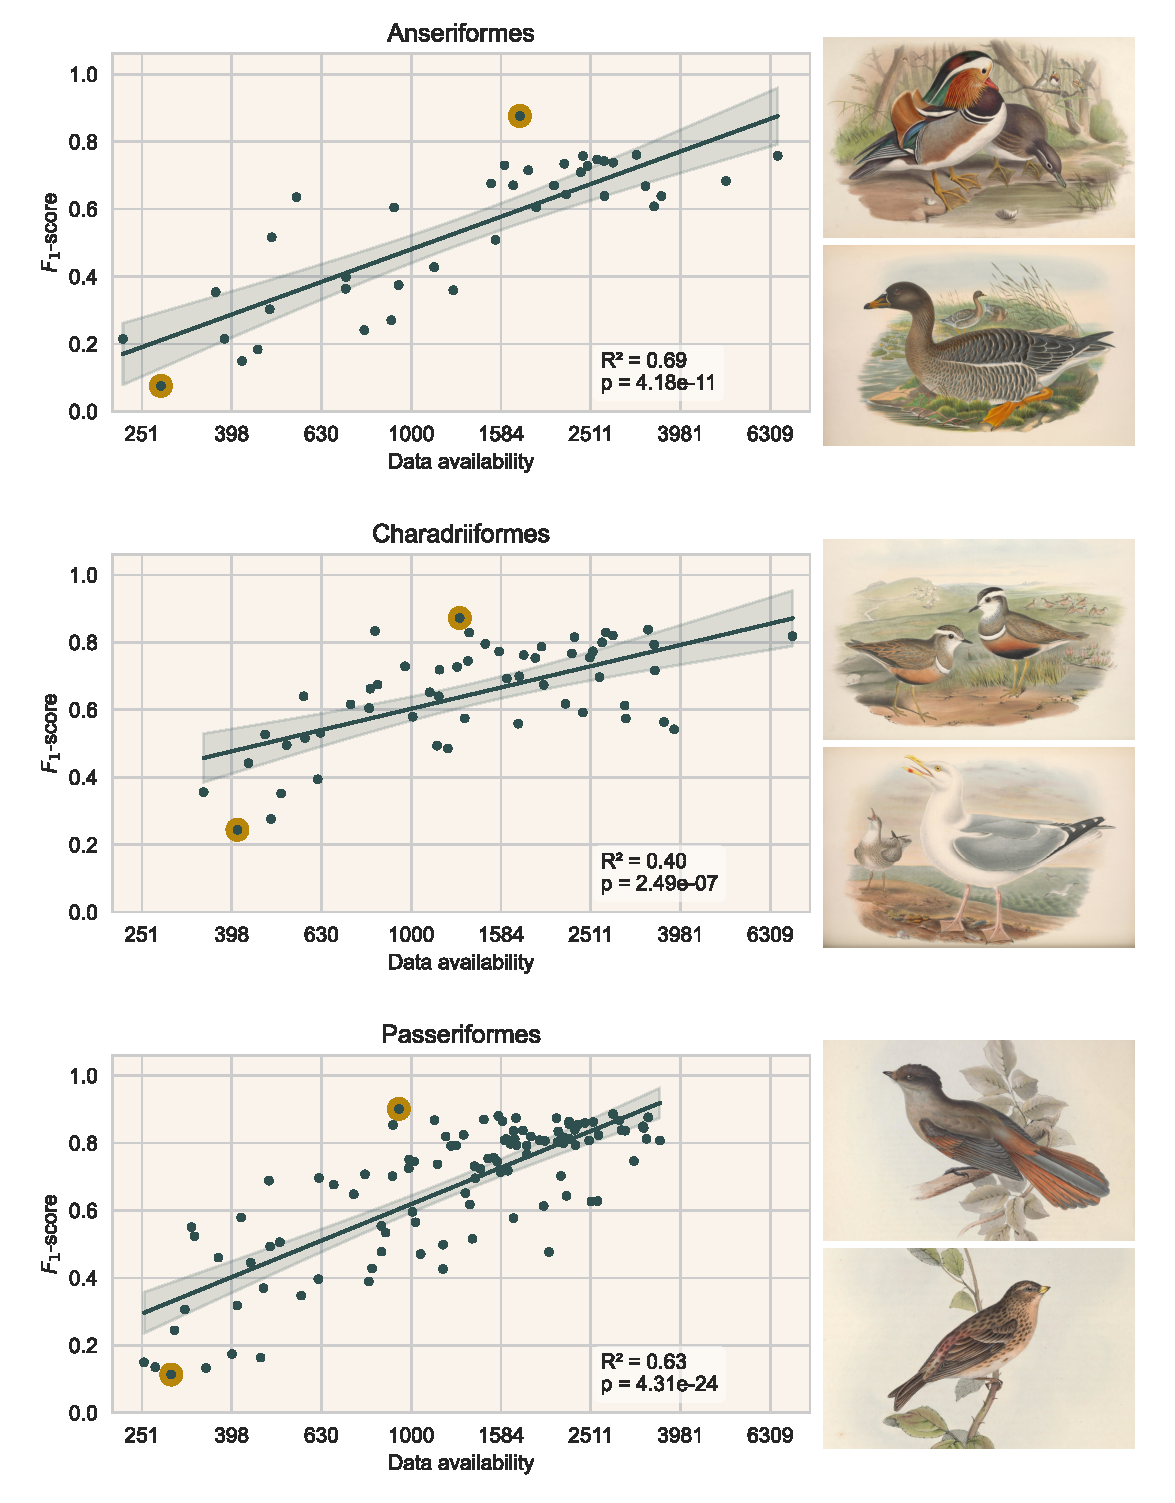
\includegraphics[width=\textwidth]{1}
  \caption{\footnotesize
    Effect of the total data availability per species on their F$_1$-scores, in models trained with 200 documented observations, for three bird orders. The top- and bottom-performing species per order (highlighted dots) are depicted, see table S1. Regressions are Ordinary Least Squares with 95\% confidence intervals.}
  \label{fig:birds}
\end{figure}


\begin{figure}[!ht]
  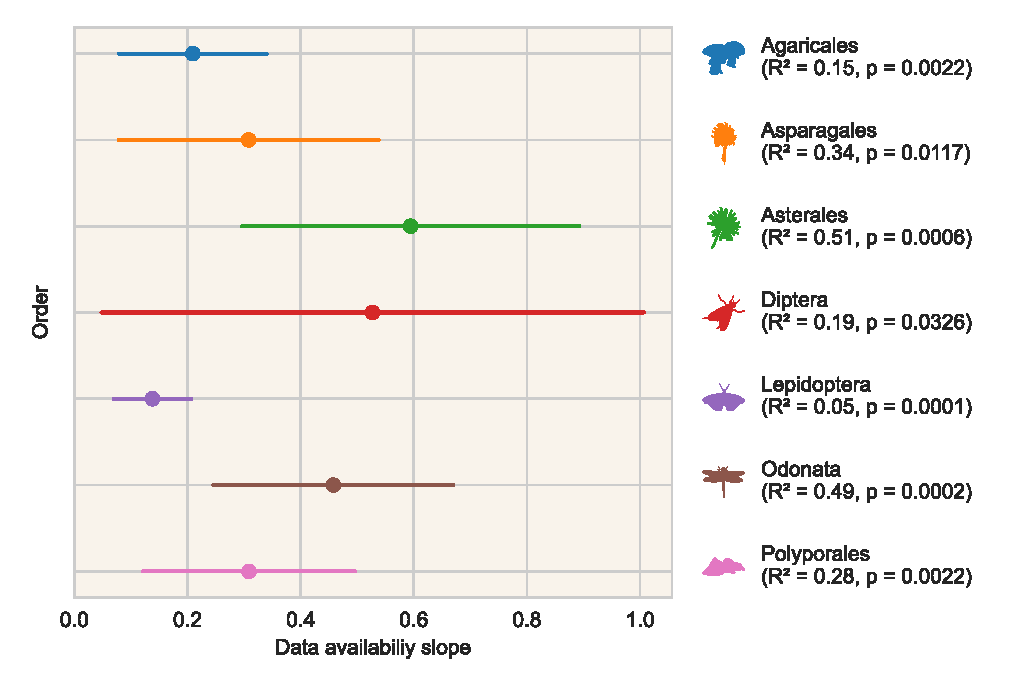
\includegraphics[width=\textwidth]{2}
  \caption{\footnotesize The slopes of the correlations between total data availability per species and their F$_1$-scores, in models trained with 200 documented observations, for non-bird orders with a correlation p$<$0.05. Regressions are Ordinary Least Squares, lines indicate the 95\% confidence intervals.}
  \label{fig:slopes}
\end{figure}

In each bird order, there is a linear relationship between species' picture density and documentation rate (R$^2$ $\geq$ 0.52, p $\leq$ 1.51×10$^{-7}$, see table S2). We also find a negative linear correlation between picture density and F$_1$-scores (R$^2$ $\geq$ 0.23, p $\leq$ 2.1×10$^{-4}$, see table S2), and some negative linear correlation between documentation rate and F$_1$-scores (R$^2$ $\geq$ 0.11, p $\leq$ 4.64×10$^{-3}$, see table S2). For passerines, there is a negative linear relationship between habitat openness and picture quality (R$^2$ = 0.26, p = 3.53×10$^{-8}$, see table S2). Waterfowl and shorebirds could not be evaluated as they only occur in open habitats.

LASSO models trained on biological traits, collection process parameters, and picture quality, all having and log data availability as an additional parameter and order as a factor, had R$^2$ values of 0.60, 0.57 and 0.63, respectively. With that, none of the full model performances were substantial improvements from a LASSO model with log data availability as its only parameter (R$^2$ =  0.57).


\section*{Discussion}
We find a conspicuous pattern where recognition models attain higher performances for species that are reported with pictures more frequently. It is probable that the recognizability of the species influences both their likelihood of being reported with pictures, as well as recognition model performances. The citizen science project used as a data source here does not include any recognition tools in its reporting or validation process, allowing a distinction between human and algorithm recognition biases. Unmistakable species can be recognized and reported by more citizen scientists, resulting in greater data availability for such species. A recognition model, dealing with the same information as human observers, is also proportionally more likely to reliably recognize these species.

This is supported by a qualitative comparison between species with the highest and lowest recognition model performances, where easy to recognize, characteristic species are reported more often than hard to recognize species (e.g. nondescript species or species similar to other related species) (see figure \ref{fig:birds} and table S1). Further support comes from the fact that most of the correlation is explained by the data availability for a species, rather than the documentation rate or the picture density. Thus, there is more data available mainly when a species is recognized and reported more, rather than it being disproportionately more likely to be reported with pictures, or with many pictures when reported with pictures.

An alternative explanation to recognizability for increased model performance might be a difference in the kind of pictures, but we find no evidence for this. Species traits, habitat use, and image quality could affect recognition model performance if pictures of more photographed birds are taken more up close, with higher zoom, or were cropped more. We found no evidence, however, for a link between model performance and either picture quality or biological traits in birds. For the passerines, where habitat openness varies among species, we do find that picture quality decreases for species associated with more open habitats. It makes intuitive sense that birds in open habitats are photographed from a greater distance than their forest dwelling counterparts, which will be hidden from view unless in close proximity. While this intercorrelation supports the validity of the picture quality metric, neither habitat nor picture quality affect recognition model performance. We conclude that differences in model performance are caused by the recognizability of the species, rather than by how, or how large species are generally depicted.

Since multiple pictures connected to a single observation are not truly independent, training data are generated based on the number of documented observations, rather than the total number of pictures. One might expect that species with a higher picture density will perform better, as observations with more pictures can provide some additional information in the training process. We find a reverse effect however, where performance for such species is substantially lower. A likely explanation is that species with high picture densities are rarities in Norway (e.g. the top 3 species being Caspian gull, Blyth's reed warbler, and Pine bunting). Species with the lowest picture density, meanwhile, are typical common, well-known species such as corvids and titmice. Rarities are reported not because they are easy to find or identify by casual observers, but due to their popularity among avid birdwatchers, who are likely to document their observations. A strong correlation between picture density and documentation rate supports this; rarities are more often reported with pictures, and in such cases relatively often with several pictures.

While we investigated the bird orders in detail, the link between data availability and model performance is present in other orders too (figure \ref{fig:slopes}). Some orders are notoriously difficult to identify to species level, e.g. flies (Diptera) and beetles (Coleoptera), but our models for these perform surprisingly well. The list of species with sufficient observations with pictures for inclusion in the experiment reveals that only relatively easy to recognize species, often with distinct colorations (e.g. ladybugs for beetles) are represented in this subset.

More generally, the requirement that species must have at least 220 citizen science observations with pictures generates a non-random subset of species, and it differs greatly per order how selective this criterion is. Bird species are most frequently reported; 48\% of the species present in Norway~\cite{NBIC} within the bird orders examined here meet the selection criterion. One of the other orders for which the pattern was found, the dragonflies and damselflies (Odonata), have only 52 species in Norway, of which 44\% met the criteria for inclusion. This is in stark contrast to the beetles (1\% inclusion), and lichens (2\% inclusion), where no clear correlation is found. It is reasonable to assume that for these taxa, the experiment only considers the most recognizable species. If observations were thousandfold, more challenging species could be included, giving a broader range in performances and possibly a similar positive correlation between model performance and data availability.

The consequence of the recognizability bias found here is that as more data is collected, ultimately providing the numbers of pictures needed to train models also on less reported, harder to recognize species, current performance of recognition models cannot be extrapolated to these expanded models. In other words, data that are lacking now are in part lacking because such species are harder to recognize. When such data is added in the future, the performance increase will not be as great as in the past. Besides citizen science, even methods that have no inherent reporting bias, such as automated insect camera traps and trail cameras, can still be subject to recognizability bias. There too, species that are less readily identified will result in more unidentifiable pictures, providing relatively less training data.

Image recognition tools play an important role in maintaining the quality of the large amounts of biodiversity data science and management require. There are limits to what can be identified from a picture however, and identification tools are needed that rely on more than just pixel information. Models that take into account season, location, sound, etc. can be especially beneficial for difficult species. Still, there is no substitute for the taxonomic knowledge of experts. Preserving this knowledge, and making it available in the form of identification keys is vital. These can be powerful tools to more reliably identify challenging species, in tandem with automatic identification.



\section*{Acknowledgements}
We are grateful to Rune Sørås, Ingeborg H. Bringslid, and Rienk W. Fokkema for their help in annotating pictures.

\section*{Data accessibility}
All code is available through Zenodo at \url{https://doi.org/10.5281/zenodo.6734696}. Bird illustrations in figure \ref{fig:birds} are works in the Public Domain made by John Gould (1804-1881), obtained through the Biodiversity Heritage Library~\cite{bhl1,bhl2,bhl3}

\section*{Authors’ contributions}
WK: conception, experimental design, code, analysis, writing. LH: code, text revision. EBN: conception, text revision. RBOH: analysis, text revision. AGF: conception, analysis, text revision.



\bibliography{Manuscript}


\newpage

\section*{Supplementary information}
\renewcommand{\thetable}{S\arabic{table}}
\setcounter{table}{0}

\begin{longtable}{|p{0.25\textwidth} | p{0.45\textwidth} | p{0.2\textwidth} |}
  \hline
  \textbf{Order}  & \textbf{Species}                       & \textbf{F$_1$-score} \\ [0.5ex]
  \hline

  Passeriformes   & \textit{Perisoreus infaustus}          & 0.901                \\ \hline
  Passeriformes   & \textit{Cinclus cinclus}               & 0.886                \\ \hline
  Passeriformes   & \textit{Periparus ater}                & 0.88                 \\ \hline
  Passeriformes   & \textit{Bombycilla garrulus}           & 0.876                \\ \hline
  Anseriformes    & \textit{Aix galericulata}              & 0.876                \\ \hline
  Passeriformes   & \textit{Certhia familiaris}            & 0.874                \\ \hline
  Passeriformes   & \textit{Aegithalos caudatus}           & 0.873                \\ \hline
  Charadriiformes & \textit{Charadrius morinellus}         & 0.872                \\ \hline
  Passeriformes   & \textit{Regulus regulus}               & 0.87                 \\ \hline
  Passeriformes   & \textit{Lophophanes cristatus}         & 0.868                \\ \hline
  Passeriformes   & \textit{Emberiza citrinella}           & 0.867                \\ \hline
  Passeriformes   & \textit{Garrulus glandarius}           & 0.865                \\ \hline
  Passeriformes   & \textit{Pyrrhula pyrrhula}             & 0.863                \\ \hline
  Passeriformes   & \textit{Pinicola enucleator}           & 0.863                \\ \hline
  Passeriformes   & \textit{Cyanistes caeruleus}           & 0.86                 \\ \hline
  Passeriformes   & \textit{Sitta europaea}                & 0.856                \\ \hline
  Passeriformes   & \textit{Turdus merula}                 & 0.855                \\ \hline
  Passeriformes   & \textit{Phylloscopus sibilatrix}       & 0.854                \\ \hline
  Passeriformes   & \textit{Coccothraustes coccothraustes} & 0.85                 \\ \hline
  Passeriformes   & \textit{Carduelis carduelis}           & 0.845                \\ \hline
  Passeriformes   & \textit{Motacilla cinerea}             & 0.839                \\ \hline
  Passeriformes   & \textit{Erithacus rubecula}            & 0.838                \\ \hline
  Passeriformes   & \textit{Parus major}                   & 0.837                \\ \hline
  Charadriiformes & \textit{Haematopus ostralegus}         & 0.837                \\ \hline
  Passeriformes   & \textit{Motacilla alba}                & 0.837                \\ \hline
  Passeriformes   & \textit{Prunella modularis}            & 0.836                \\ \hline
  Passeriformes   & \textit{Lanius collurio}               & 0.835                \\ \hline
  Charadriiformes & \textit{Phalaropus lobatus}            & 0.834                \\ \hline
  Charadriiformes & \textit{Calidris maritima}             & 0.83                 \\ \hline
  Charadriiformes & \textit{Arenaria interpres}            & 0.829                \\ \hline
  Passeriformes   & \textit{Phylloscopus inornatus}        & 0.824                \\ \hline
  Passeriformes   & \textit{Saxicola rubicola}             & 0.823                \\ \hline
  Charadriiformes & \textit{Charadrius hiaticula}          & 0.82                 \\ \hline
  Passeriformes   & \textit{Sylvia atricapilla}            & 0.82                 \\ \hline
  Passeriformes   & \textit{Turdus philomelos}             & 0.819                \\ \hline
  Charadriiformes & \textit{Gallinago gallinago}           & 0.819                \\ \hline
  Passeriformes   & \textit{Luscinia svecica}              & 0.818                \\ \hline
  Passeriformes   & \textit{Plectrophenax nivalis}         & 0.816                \\ \hline
  Charadriiformes & \textit{Tringa totanus}                & 0.815                \\ \hline
  Passeriformes   & \textit{Lanius excubitor}              & 0.813                \\ \hline
  Passeriformes   & \textit{Turdus viscivorus}             & 0.812                \\ \hline
  Passeriformes   & \textit{Fringilla coelebs}             & 0.812                \\ \hline
  Passeriformes   & \textit{Nucifraga caryocatactes}       & 0.812                \\ \hline
  Passeriformes   & \textit{Passer montanus}               & 0.808                \\ \hline
  Passeriformes   & \textit{Turdus iliacus}                & 0.808                \\ \hline
  Passeriformes   & \textit{Emberiza schoeniclus}          & 0.808                \\ \hline
  Passeriformes   & \textit{Oenanthe oenanthe}             & 0.807                \\ \hline
  Passeriformes   & \textit{Saxicola rubetra}              & 0.807                \\ \hline
  Passeriformes   & \textit{Chloris chloris}               & 0.802                \\ \hline
  Charadriiformes & \textit{Calidris alpina}               & 0.8                  \\ \hline
  Passeriformes   & \textit{Anthus petrosus}               & 0.8                  \\ \hline
  Passeriformes   & \textit{Motacilla flava}               & 0.798                \\ \hline
  Charadriiformes & \textit{Cepphus grylle}                & 0.795                \\ \hline
  Passeriformes   & \textit{Fringilla montifringilla}      & 0.794                \\ \hline
  Passeriformes   & \textit{Troglodytes troglodytes}       & 0.794                \\ \hline
  Charadriiformes & \textit{Vanellus vanellus}             & 0.793                \\ \hline
  Passeriformes   & \textit{Carpodacus erythrinus}         & 0.793                \\ \hline
  Passeriformes   & \textit{Turdus torquatus}              & 0.793                \\ \hline
  Passeriformes   & \textit{Eremophila alpestris}          & 0.792                \\ \hline
  Charadriiformes & \textit{Actitis hypoleucos}            & 0.788                \\ \hline
  Charadriiformes & \textit{Pluvialis apricaria}           & 0.773                \\ \hline
  Charadriiformes & \textit{Tringa glareola}               & 0.773                \\ \hline
  Charadriiformes & \textit{Limosa lapponica}              & 0.767                \\ \hline
  Passeriformes   & \textit{Ficedula hypoleuca}            & 0.766                \\ \hline
  Charadriiformes & \textit{Charadrius dubius}             & 0.762                \\ \hline
  Anseriformes    & \textit{Cygnus olor}                   & 0.761                \\ \hline
  Anseriformes    & \textit{Mergellus albellus}            & 0.758                \\ \hline
  Anseriformes    & \textit{Clangula hyemalis}             & 0.757                \\ \hline
  Passeriformes   & \textit{Muscicapa striata}             & 0.756                \\ \hline
  Charadriiformes & \textit{Calidris pugnax}               & 0.755                \\ \hline
  Passeriformes   & \textit{Phoenicurus ochruros}          & 0.754                \\ \hline
  Charadriiformes & \textit{Tringa nebularia}              & 0.754                \\ \hline
  Passeriformes   & \textit{Acrocephalus schoenobaenus}    & 0.751                \\ \hline
  Anseriformes    & \textit{Branta leucopsis}              & 0.747                \\ \hline
  Passeriformes   & \textit{Sturnus vulgaris}              & 0.746                \\ \hline
  Charadriiformes & \textit{Limosa limosa}                 & 0.745                \\ \hline
  Passeriformes   & \textit{Calcarius lapponicus}          & 0.745                \\ \hline
  Passeriformes   & \textit{Phoenicurus phoenicurus}       & 0.744                \\ \hline
  Anseriformes    & \textit{Mergus merganser}              & 0.742                \\ \hline
  Anseriformes    & \textit{Bucephala clangula}            & 0.738                \\ \hline
  Passeriformes   & \textit{Curruca communis}              & 0.737                \\ \hline
  Anseriformes    & \textit{Tadorna tadorna}               & 0.734                \\ \hline
  Passeriformes   & \textit{Poecile montanus}              & 0.732                \\ \hline
  Anseriformes    & \textit{Melanitta fusca}               & 0.73                 \\ \hline
  Charadriiformes & \textit{Tringa erythropus}             & 0.729                \\ \hline
  Anseriformes    & \textit{Anas acuta}                    & 0.728                \\ \hline
  Charadriiformes & \textit{Calidris minuta}               & 0.727                \\ \hline
  Passeriformes   & \textit{Poecile palustris}             & 0.725                \\ \hline
  Passeriformes   & \textit{Passer domesticus}             & 0.723                \\ \hline
  Charadriiformes & \textit{Calidris temminckii}           & 0.719                \\ \hline
  Passeriformes   & \textit{Hirundo rustica}               & 0.718                \\ \hline
  Charadriiformes & \textit{Numenius arquata}              & 0.716                \\ \hline
  Anseriformes    & \textit{Mareca penelope}               & 0.715                \\ \hline
  Passeriformes   & \textit{Corvus frugilegus}             & 0.714                \\ \hline
  Anseriformes    & \textit{Mergus serrator}               & 0.71                 \\ \hline
  Passeriformes   & \textit{Sylvia curruca}                & 0.708                \\ \hline
  Passeriformes   & \textit{Turdus pilaris}                & 0.703                \\ \hline
  Passeriformes   & \textit{Pica pica}                     & 0.702                \\ \hline
  Charadriiformes & \textit{Uria aalge}                    & 0.699                \\ \hline
  Charadriiformes & \textit{Chroicocephalus ridibundus}    & 0.697                \\ \hline
  Passeriformes   & \textit{Hippolais icterina}            & 0.696                \\ \hline
  Passeriformes   & \textit{Loxia leucoptera}              & 0.696                \\ \hline
  Charadriiformes & \textit{Calidris canutus}              & 0.693                \\ \hline
  Passeriformes   & \textit{Emberiza pusilla}              & 0.688                \\ \hline
  Anseriformes    & \textit{Cygnus cygnus}                 & 0.683                \\ \hline
  Passeriformes   & \textit{Panurus biarmicus}             & 0.677                \\ \hline
  Anseriformes    & \textit{Somateria spectabilis}         & 0.676                \\ \hline
  Charadriiformes & \textit{Alca torda}                    & 0.675                \\ \hline
  Charadriiformes & \textit{Rissa tridactyla}              & 0.674                \\ \hline
  Anseriformes    & \textit{Branta canadensis}             & 0.671                \\ \hline
  Anseriformes    & \textit{Aythya fuligula}               & 0.67                 \\ \hline
  Anseriformes    & \textit{Anas platyrhynchos}            & 0.668                \\ \hline
  Charadriiformes & \textit{Alle alle}                     & 0.663                \\ \hline
  Charadriiformes & \textit{Calidris alba}                 & 0.652                \\ \hline
  Passeriformes   & \textit{Alauda arvensis}               & 0.651                \\ \hline
  Passeriformes   & \textit{Corvus monedula}               & 0.648                \\ \hline
  Anseriformes    & \textit{Anas crecca}                   & 0.644                \\ \hline
  Passeriformes   & \textit{Phylloscopus collybita}        & 0.643                \\ \hline
  Charadriiformes & \textit{Pluvialis squatarola}          & 0.64                 \\ \hline
  Charadriiformes & \textit{Fratercula arctica}            & 0.64                 \\ \hline
  Anseriformes    & \textit{Somateria mollissima}          & 0.639                \\ \hline
  Anseriformes    & \textit{Anser anser}                   & 0.639                \\ \hline
  Anseriformes    & \textit{Anser indicus}                 & 0.635                \\ \hline
  Passeriformes   & \textit{Acanthis flammea}              & 0.628                \\ \hline
  Passeriformes   & \textit{Anthus pratensis}              & 0.627                \\ \hline
  Charadriiformes & \textit{Sterna hirundo}                & 0.618                \\ \hline
  Passeriformes   & \textit{Corvus cornix}                 & 0.618                \\ \hline
  Charadriiformes & \textit{Stercorarius parasiticus}      & 0.616                \\ \hline
  Passeriformes   & \textit{Phylloscopus trochilus}        & 0.613                \\ \hline
  Charadriiformes & \textit{Larus hyperboreus}             & 0.613                \\ \hline
  Anseriformes    & \textit{Anser brachyrhynchus}          & 0.608                \\ \hline
  Anseriformes    & \textit{Aythya marila}                 & 0.605                \\ \hline
  Charadriiformes & \textit{Calidris ferruginea}           & 0.605                \\ \hline
  Anseriformes    & \textit{Aythya ferina}                 & 0.605                \\ \hline
  Passeriformes   & \textit{Corvus corax}                  & 0.596                \\ \hline
  Charadriiformes & \textit{Larus fuscus}                  & 0.592                \\ \hline
  Charadriiformes & \textit{Tringa ochropus}               & 0.58                 \\ \hline
  Passeriformes   & \textit{Locustella naevia}             & 0.579                \\ \hline
  Passeriformes   & \textit{Carduelis spinus}              & 0.577                \\ \hline
  Charadriiformes & \textit{Numenius phaeopus}             & 0.575                \\ \hline
  Charadriiformes & \textit{Larus canus}                   & 0.574                \\ \hline
  Passeriformes   & \textit{Carduelis flavirostris}        & 0.565                \\ \hline
  Charadriiformes & \textit{Larus glaucoides}              & 0.564                \\ \hline
  Charadriiformes & \textit{Larus marinus}                 & 0.559                \\ \hline
  Passeriformes   & \textit{Anthus trivialis}              & 0.554                \\ \hline
  Passeriformes   & \textit{Regulus ignicapilla}           & 0.55                 \\ \hline
  Charadriiformes & \textit{Larus argentatus}              & 0.542                \\ \hline
  Passeriformes   & \textit{Riparia riparia}               & 0.534                \\ \hline
  Charadriiformes & \textit{Scolopax rusticola}            & 0.532                \\ \hline
  Charadriiformes & \textit{Phalaropus fulicarius}         & 0.526                \\ \hline
  Passeriformes   & \textit{Sylvia nisoria}                & 0.523                \\ \hline
  Anseriformes    & \textit{Polysticta stelleri}           & 0.517                \\ \hline
  Passeriformes   & \textit{Acanthis hornemanni}           & 0.516                \\ \hline
  Charadriiformes & \textit{Stercorarius skua}             & 0.516                \\ \hline
  Anseriformes    & \textit{Melanitta nigra}               & 0.509                \\ \hline
  Passeriformes   & \textit{Sylvia borin}                  & 0.506                \\ \hline
  Passeriformes   & \textit{Loxia pytyopsittacus}          & 0.498                \\ \hline
  Charadriiformes & \textit{Calidris falcinellus}          & 0.495                \\ \hline
  Charadriiformes & \textit{Sterna paradisaea}             & 0.493                \\ \hline
  Passeriformes   & \textit{Lullula arborea}               & 0.493                \\ \hline
  Charadriiformes & \textit{Hydrocoloeus minutus}          & 0.485                \\ \hline
  Passeriformes   & \textit{Pastor roseus}                 & 0.478                \\ \hline
  Passeriformes   & \textit{Loxia curvirostra}             & 0.477                \\ \hline
  Passeriformes   & \textit{Acanthis cabaret}              & 0.471                \\ \hline
  Passeriformes   & \textit{Turdus atrogularis}            & 0.46                 \\ \hline
  Passeriformes   & \textit{Ficedula parva}                & 0.445                \\ \hline
  Charadriiformes & \textit{Stercorarius longicaudus}      & 0.442                \\ \hline
  Passeriformes   & \textit{Corvus corone}                 & 0.428                \\ \hline
  Anseriformes    & \textit{Anas clypeata}                 & 0.428                \\ \hline
  Passeriformes   & \textit{Carduelis cannabina}           & 0.426                \\ \hline
  Anseriformes    & \textit{Anser albifrons}               & 0.399                \\ \hline
  Passeriformes   & \textit{Acrocephalus dumetorum}        & 0.397                \\ \hline
  Charadriiformes & \textit{Calidris melanotos}            & 0.394                \\ \hline
  Passeriformes   & \textit{Acrocephalus palustris}        & 0.389                \\ \hline
  Anseriformes    & \textit{Anas strepera}                 & 0.375                \\ \hline
  Passeriformes   & \textit{Delichon urbicum}              & 0.37                 \\ \hline
  Anseriformes    & \textit{Mareca strepera}               & 0.364                \\ \hline
  Anseriformes    & \textit{Anser fabalis}                 & 0.359                \\ \hline
  Charadriiformes & \textit{Thalasseus sandvicensis}       & 0.356                \\ \hline
  Anseriformes    & \textit{Branta bernicla}               & 0.354                \\ \hline
  Charadriiformes & \textit{Larus melanocephalus}          & 0.352                \\ \hline
  Passeriformes   & \textit{Acrocephalus scirpaceus}       & 0.347                \\ \hline
  Passeriformes   & \textit{Motacilla citreola}            & 0.318                \\ \hline
  Passeriformes   & \textit{Luscinia luscinia}             & 0.307                \\ \hline
  Anseriformes    & \textit{Aythya collaris}               & 0.303                \\ \hline
  Charadriiformes & \textit{Lymnocryptes minimus}          & 0.276                \\ \hline
  Anseriformes    & \textit{Spatula clypeata}              & 0.271                \\ \hline
  Passeriformes   & \textit{Emberiza leucocephalos}        & 0.244                \\ \hline
  Charadriiformes & \textit{Larus cachinnans}              & 0.244                \\ \hline
  Anseriformes    & \textit{Anas querquedula}              & 0.241                \\ \hline
  Anseriformes    & \textit{Anas carolinensis}             & 0.215                \\ \hline
  Anseriformes    & \textit{Tadorna ferruginea}            & 0.215                \\ \hline
  Anseriformes    & \textit{Cygnus columbianus}            & 0.184                \\ \hline
  Passeriformes   & \textit{Anthus richardi}               & 0.174                \\ \hline
  Passeriformes   & \textit{Spinus spinus}                 & 0.164                \\ \hline
  Passeriformes   & \textit{Anthus hodgsoni}               & 0.15                 \\ \hline
  Anseriformes    & \textit{Spatula querquedula}           & 0.149                \\ \hline
  Passeriformes   & \textit{Anthus cervinus}               & 0.136                \\ \hline
  Passeriformes   & \textit{Linaria cannabina}             & 0.133                \\ \hline
  Passeriformes   & \textit{Linaria flavirostris}          & 0.113                \\ \hline
  Anseriformes    & \textit{Anser serrirostris}            & 0.076                \\ \hline


  \caption{\footnotesize Metrics collected for species within the bird orders}
  \label{tab:birdscores}
\end{longtable}




\begin{longtable}{|p{0.20\textwidth} | p{0.20\textwidth} | p{0.08\textwidth} | p{0.13\textwidth} | p{0.05\textwidth} | p{0.135\textwidth} |}
  \hline
  \textbf{Dependent variable}        &
  \textbf{Parameters}                &
  \textbf{Slope}                     &
  \textbf{Intercept}                 &
  \textbf{R$^2$}                     &
  \textbf{P-value}                                                                                      \\ [0.5ex]
  \hline

  Agaricales F$_1$-score             & Data availability (log) & 0.21  & 0.27  & 0.15 & 2.15×10$^{-3}$  \\ \hline
  Anseriformes documentation rate    & Picture density         & 0.38  & -0.47 & 0.52 & 1.51×10$^{-7}$  \\ \hline
  Anseriformes F$_1$-score           & Data availability (log) & 0.48  & -0.97 & 0.69 & 4.18×10$^{-11}$ \\ \hline
  Anseriformes F$_1$-score           & Documentation rate      & -1.52 & 0.63  & 0.19 & 4.64×10$^{-3}$  \\ \hline
  Anseriformes F$_1$-score           & Picture density         & -1.02 & 1.95  & 0.31 & 2.10×10$^{-4}$  \\ \hline
  Asparagales F$_1$-score            & Data availability (log) & 0.31  & 0.01  & 0.34 & 0.0117          \\ \hline
  Asterales F$_1$-score              & Data availability (log) & 0.59  & -0.71 & 0.51 & 5.92×10$^{-4}$  \\ \hline
  Charadriiformes documentation rate & Picture density         & 0.34  & -0.43 & 0.76 & 5.51×10$^{-18}$ \\ \hline
  Charadriiformes F$_1$-score        & Data availability (log) & 0.32  & -0.34 & 0.4  & 2.49×10$^{-7}$  \\ \hline
  Charadriiformes F$_1$-score        & Documentation rate      & -0.9  & 0.7   & 0.28 & 3.45×10$^{-5}$  \\ \hline
  Charadriiformes F$_1$-score        & Picture density         & -0.42 & 1.25  & 0.39 & 3.52×10$^{-7}$  \\ \hline
  Coleoptera F$_1$-score             & Data availability (log) & 0.13  & 0.57  & 0.06 & 0.273           \\ \hline
  Diptera F$_1$-score                & Data availability (log) & 0.53  & -0.63 & 0.19 & 0.0326          \\ \hline
  Lecanorales F$_1$-score            & Data availability (log) & 0.2   & 0.31  & 0.12 & 0.118           \\ \hline
  Lepidoptera F$_1$-score            & Data availability (log) & 0.14  & 0.49  & 0.05 & 9.50×10$^{-5}$  \\ \hline
  Odonata F$_1$-score                & Data availability (log) & 0.46  & -0.53 & 0.49 & 2.02×10$^{-4}$  \\ \hline
  Passeriformes documentation rate   & Picture density         & 0.3   & -0.36 & 0.55 & 1.59×10$^{-19}$ \\ \hline
  Passeriformes F$_1$-score          & Data availability (log) & 0.54  & -1    & 0.63 & 4.31×10$^{-24}$ \\ \hline
  Passeriformes F$_1$-score          & Documentation rate      & -0.85 & 0.71  & 0.11 & 5.19×10$^{-4}$  \\ \hline
  Passeriformes F$_1$-score          & Picture density         & -0.5  & 1.37  & 0.23 & 1.68×10$^{-7}$  \\ \hline
  Passeriformes picture quality      & Habitat openness        & -0.12 & 5.93  & 0.26 & 5.53×10$^{-8}$  \\ \hline
  Polyporales F$_1$-score            & Data availability (log) & 0.31  & -0.11 & 0.28 & 2.18×10$^{-3}$  \\ \hline

  \hline


  \caption{\footnotesize Metrics collected for species within the bird orders}
  \label{tab:stats}
\end{longtable}


\end{document}